\begin{abstract}
The most promising technology expected to alleviate the intra-chip and chip-to-chip interconnection bottleneck is silicon photonics, in which electronics and photonics can be integrated monolithically, only requiring standard CMOS processing lines for fabrication. Nonlinear interaction can provide all-optical processing capabilities, which do not have the bandwidth limitations imposed by electronics. Silicon has a Kerr coefficient which is 100 times higher than silica; this fact, together with the strong confinement because its high refractive index difference, makes nonlinear effects take place at relatively low optical powers.

However, at $1.5~\mu$m, silicon undergoes two-photon absorption too, generating carriers with slower dynamics that can mask the ultrafast nonlinear Kerr effect. There are different strategies to reduce the effect of carriers, such as carrier sweeping through a PN junction or reduction of carrier lifetime through introduction of recombination centers. Another possibility is using a slot waveguide, with most light confined in the slot and not in the silicon, allows having a highly nonlinear material inside the slot, such as silicon nanocrystals ~\cite{Oton2010,Matres2011,Matres:12}. Amorphous silicon should also be considered because its high nonlinearity and low carrier effects~\cite{Matres2013}. In this thesis, we consider all these different materials, waveguides and devices (ring resonator and Mach Zehnder interferometer) for making all-optical switches that can work at 40~Gb/s bitrates or higher.
\end{abstract}


\begin{abstract}
La tecnología más prometedora para solventar el cuello de botella en las actuales interconexiones entre chips y dentro del chip es la fotónica en silicio, donde la electrónica y la fotónica pueden integrarse monolíticamente, requiriendo solamente un proceso estándar de fabricacion CMOS.
Además, la interacción no lineal proporciona al silicio capacidades de procesamiento todo-óptico, sin limitaciones de ancho de banda como las que sufre la electrónica.
El silicio tiene un coeficiente Kerr 100 veces mayor que la sílice; este hecho, junto con el gran confinamiento debido al alto contraste de índice de refracción, permite observar efectos no lineales a potencias ópticas relativamente bajas.

Sin embargo, a 1,5 micras de longitud de onda el silicio sufre un efecto conocido como absorción de dos fotones. Esta generación de portadores tiene una dinámica más lenta que puede enmascarar el efecto kerr ultrarrápido.
Para reducir el efecto de los portadores suelen utilizarse distintas estrategias, tales como barrer portadores a través de una unión PN o reducir el tiempo de vida de los portadores introduciendo de centros de recombinación. Otra posibilidad es usar una guía de onda ranurada, en las que el modo se confina en la ranura en vez de en el silicio ~\cite{Oton2010,Matres2011,Matres:12}. También hemos de considerar el Silicio amorfo, por su alta no linealidad y menores efectos de portadores~\cite{Matres2013}. En esta tesis, se consideran todas estas guías de onda y estructuras (anillo resonante o MZI) para la fabricación de conmutadores totalmente ópticos a velocidades por encima de 40 Gb/s.
\end{abstract}


\begin{abstract}
La tecnologia més prometedora per les futures interconnexions intra-xip i de xip a xip és la fotònica de silici, en què l'electrònica i la fotònica s'integren monolíticament, només requerint línies de procés CMOS estàndard per a la fabricació. L' interacció no lineal pot proporcionar capacitats de processament totalment òptiques, sense les limitacions d'ample de banda imposades per l'electrònica. El silici té un coeficient de Kerr, que és 100 vegades més gran que la sílice, aquest fet, juntament amb el fort confinament a causa de la gran diferència d'índex de refracció, permeteix utilitzar efectes no lineals amb una potencia òptica relativament baixa.

No obstant això, a 1,5 micres de longitud d'ona, el silici també es sotmet a l'absorció de dos fotons, generant portadors amb dinàmica més lenta que poden emmascarar l'efecte no lineal Kerr ultraràpid. Hi ha diferents estratègies per reduir l'efecte dels portadors, com accelerar portadors a través d'una unió PN o reduir el temps de vida dels portadors a través de la introducció de centres de recombinació. Una altra possibilitat és utilitzar una guia ranurada, amb la majoria de la llum confinat a la ranura i no en el silici ~\cite{Oton2010,Matres2011,Matres:12}. El silici amorf també ha de ser considerat, per la seva alta no linealitat i baixos efectes de portadors~\cite{Matres2013}. En aquesta tesi, es consideren totes aquestes guies d'ona i estructures (anell resonant o MZI) per a la fabricació de commutadors totalment òptics a velocitats de 40 Gb/s o superiors.
\end{abstract}

\pagestyle{fancy}
\lhead{}
\renewcommand{\chaptermark}[1]{\markboth{\thechapter.\ #1}{}}
\pagenumbering{arabic}
\chapter{Introduction}
\label{ch:intro}

In recent years, telecommunication technologies have experienced a great development. This increase is due to the growing number of users, which at the same time makes networks more attractive for the creation of innovative and sophisticated applications.
To meet the needs of these applications, large capacity communications networks interconnection are required, which have resulted in major impacts on society.
These two factors, both the increasing number of users and the emergence of more sophisticated applications, has forced the networks to evolve, so that communication needs can be met.


\section{Optical Technology}
To meet our basic need to communicate, new technologies have appeared to achieve the maximum bandwidth at reasonable prices.
It is then when optical technology begins to be used between core network nodes, mainly in the form of single-mode fiber links.
This links have a bandwidth of several Gbit/s per wavelength, which in total can aggregate a total capacity of over 1 Tbit/s.
However, the main functions of these network nodes, such as routing, are still being done in the electrical domain, which is a major bottleneck for the future.
Currently we are trying to develop optical technology in the network nodes in order to develop high performance optical networks.


\begin{figure}[htb]
	\centering
	\includegraphics[width=0.60\textwidth]{mux}
	\caption{Multiplexing information in different wavelengths we can reach Tbit/s capacity with a single optical waveguide. (Intel)}
\end{figure}


\section{Integrated optics}
The best strategy to manufacture optical devices with different functions, high bandwidth and low cost is to use integrated optics, in which a single manufacturing process can generate large volumes of production, resulting in a dramatic decrease of the cost per device.

Currently, the main technologies used for manufacturing integrated optical devices are based on group III-V elements such as Indium Phosphide (InP) and gallium arsenide (GaAs) that can monolithically integrate active components such as lasers and amplifiers, lithium niobate ($ \mathrm{LiNbO_3} $) for high performance external modulators and doped glasses for low scale of integration passive components (Arrayed Waveguide Gratings, etc.).
These materials have very good optical properties and many global companies, such as JDS Uniphase and Bookham, have developed commercial optical devices such as lasers, modulators and multiplexers/demultiplexers for WDM networks. However, these materials require highly specialized manufacturing technologies, and are not suitable for large-scale manufacturing.

With the increasing demand of bandwidth, optical links start to become necessary for lower distances, getting closer to the electronic circuits in data centers. Therefore, there is a great need to reduce the cost of optical devices in this new datacom emerging market, with more growing prospects for optical communications than the traditional telecom market.


\section{Silicon Integrated optics}
The most developed manufacturing processes are the Complementary Metal Oxide Semiconductor (CMOS), highly developed during many years by the microelectronics industry.
Unfortunately, III-V technologies are not compatible with CMOS, and their manufacturing processes are not as mature and developed.
In this way, it is necessary to investigate new optical technologies that allow the development of high performance commercial prototypes compatible with CMOS manufacturing processes.
This is how the development of silicon photonic technologies will allow mass production of optical devices at a lower cost.

In addition, silicon is transparent in the two telecommunication wavelengths, which are at 1.3 and 1.55 microns. Moreover the high index difference between silicon (3.47) and silica (1.44) at those particular wavelengths, allows the confinement of light in very small waveguides, below one micron, and very small bending radius, allowing a drastic reduction of the area required by the device in the wafer and a very high degree of integration. Finally, the high degree of confinement enables using nonlinear optical effects at moderate powers, allowing the realization of all-optical devices.

Silicon photonics is now a reality, and the proof is that companies like IBM, Intel, Luxtera and Kotura are currently manufacturing silicon photonic devices using CMOS-compatible technology. These devices are primarily modulators, detectors and sensors.
The main problem of the silicon optical devices is the difficulty of achieving efficient light emission and amplification due to its indirect gap.
On the other hand, the powers necessary to obtain non-linear effects also generate carriers in the silicon that hinder the realization of ultrafast devices.
At present, research centers and major global companies are putting great efforts in developing nonlinear active devices in silicon, and the proof is the large number of very high impact publications made in recent years.~\cite{Reed2004,Almeida2004b,Boyraz2004,Preble2005,Liang:05,Hochberg2006,Jacobsen2006,Foster2007,Waldow2008,Lee2009,koos2009}


\section{Objective}
The objective is this thesis is to study different strategies for a high speed and low cost solution for future optical interconnects. All optical switching will allow us to increase the speed using ultrafast nonlinear kerr effect and scale the power needed. Moreover all the materials considered are compatible with CMOS technology, which is crucial for large scale manufacturing at competitive prices.


\section{Methodology}
\label{ch:methodology}
Three main activities necessary for this dissertation were:

\subsection{Design}
It required the use of simulation tools to predict the optical properties of the waveguides and devices. Depending on the characteristics of the device (optical waveguides, couplers, resonators, etc.) there are different simulation methods that are more suitable for each design (See appendix~\ref{ch:simulations}).

\begin{figure}[htb]
  \centering
  \includegraphics[width=0.49\textwidth]{out_resonance}              
  \includegraphics[width=0.49\textwidth]{in_resonance}
  \caption{FDTD simulation of a 20~$\mu$m radius resonator at 1.55~$\mu$m. Light only passes through when the ring is out of resonance. Waveguides were made of fully etched Silicon (3.47), with 220~nm height and 500~nm width, surrounded by Silica (1.44). The gap between the ring and the waveguide was 200~nm and light polarization was set to TE.
  }
\end{figure}

\subsection{Fabrication}
The Valencia Nanophotonics Technology Center has $ 500~\mathrm{m}^2 $ of clean-rooms and all the necessary equipment to fabricate optical integrated circuits. The most important techniques available include electron beam lithography, inductively coupled plasma reactive ion etching, oxide and poly-silicon deposition, electron microscopy, etc.
The fabrication processes were carried out by specialized engineers of the Institute and we also collaborated with the most advanced research centers in Europe. Particularly, we worked in several European projects with CEA-LETI and IMEC, allowing us to design samples that required processes not available in Valencia.

\begin{figure}[htb]
  \centering
  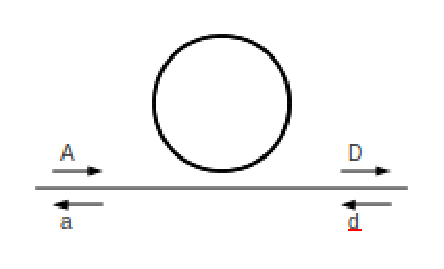
\includegraphics[width=0.49\textwidth]{anillo}              
  \includegraphics[width=0.49\textwidth]{SEM}
  \caption{Electron microscopy image of a ring resonator fabricated in our facilities. Starting from SOI wafers with 3~$\mu m$ buried oxide and 250~nm silicon layer, waveguides were patterned with e-beam lithography and etched with an inductively coupled plasma (ICP) etcher. The structures were covered with 2~$\mu m$ of silica after SEM characterization. The channels were 500~nm wide and 250~nm high, and were coupled to a 10~$\mu m$-radius ring through a 300~nm gap.
  }

\end{figure}


\subsection{Testing}
Devices were tested in fully equipped laboratories, with capacity of ultrafast nonlinear measurements. For this, the center has several laser sources (tunable, pulsed and continuous) in the range of 1.3-1.6 microns, coupling systems (fiber, objective or grating), and detection systems with bandwidths above 40~GHz. Nonlinear experiments include pump and probe measurements, where a pump generates changes in the propagation of a signal by cross-absorption-modulation (XAM) and cross-phase-modulation (XPM). These changes can be exploited for all-optical switching and logic gates (Section~\ref{ch:allOpticalSwitching}). For this, I used Mach-Zehnder interferometers or ring resonators to convert phase modulation into amplitude modulation.
Finally, I characterized the lifetime of the carriers (\ref{ch:timeRes}), which is decisive to determine the maximum switching speed of the devices and investigated parametric processes such as four wave mixing, as it has recently been shown that, under certain conditions, it can be efficient in silicon guides (\ref{ch:fwm}).


\begin{figure}[htb]
  \centering
  \includegraphics[width=0.49\textwidth]{horizontal2}            
  \includegraphics[width=0.49\textwidth]{vertical2}
  \caption{Horizontal and vertical coupling setups for sample characterization.}
\end{figure}



\section{Outline}
Chapter~\ref{ch:PhotonicCircuits} introduces the building blocks and chapter~\ref{ch:nonlinearEffects} the nonlinear effects that play a role for developing all-optical switches.
Chapters~\ref{ch:paperSwitching}-\ref{ch:paperLogicGates} present an all optical switch and a logic gate, using a microring resonator and a Mach Zehnder Interferometer respectively.
Chapters~\ref{ch:articleTimeRes}-\ref{ch:articleFigureOfMerit} characterize the figures of merit of different nonlinear waveguides.
Then, appendix~\ref{ch:experimentalSetups} describes the different experimental setups, where Ref.~\ref{ch:paperBackscattering} presents a technique to characterize rings that considers backscattering effects through a model and Ref.~\ref{ch:paperPhase} is a technique to measure the phase of different devices. Finally, appendix~\ref{ch:simulations} covers different simulation algorithms used for this dissertation.


\pagestyle{plain}
\bibliographystyle{unsrt}
\bibliography{library}

